\chapter{Implementierung}
Nachdem nun die erwarteten Funktionen festgelegt sind, soll in diesem Kapitel die genauere Implementierung vorgestellt werden. Hierbei wird auch auf eine mögliche Erweiterbarkeit des Bots eingegangen.

Der Source Code des Bots ist auf Github über die Adresse \url{https://github.com/TobsCore/IWINewsBot} zu finden. Von dort aus kann der Code über den folgenden Befehl geladen werden.

\begin{lstlisting}
git clone https://github.com/TobsCore/IWINewsBot
\end{lstlisting}

In dem geladenen Ordner \texttt{IWINewsBot} befinden sich dabei die folgenden drei Ordner: \texttt{src}, \texttt{project} und \texttt{Documentation}. In \texttt{src/} sind die Dateien für den Bot enthalten, in \texttt{project/} befinden sich Informationen zu dem SBT-Projekt und in \texttt{Documentation} sind die Quelldateien für diese Dokumentation enthalten.

Damit der Bot korrekt starten kann, ist ein Token notwendig, hierzu legt man im Root-Ordner die Datei \texttt{bot.token} an und speichert in dieser Datei das vom BotFather generierte Token. Der Bot wird diese Datei dann nutzen, um sich zu verifizieren. Aus Sicherheitsgründen ist das Token nicht im Repository gespeichert.

\section{Scala und das Scala Build Tool}
Es wurde entschieden, den Bot in Scala zu programmieren, da dies eine interessante Programmiersprache ist, mit der man als Studierender nicht viele Berührungspunkte hat. Scala bietet durch die Objektorientierung vertraute Konzepte, jedoch sind viele Konzepte der funktionalen Programmierung in der Sprache vorhanden.

Um das Projekt zuverlässig bauen zu können und Abhängigkeiten zu verwalten, wird das Scala-Build-Tool (kurz \emph{SBT}) eingesetzt. Dieses Build-Tool gilt als Standard-Build-Tool für Scala Projekte. Um das Projekt besser kennen lernen zu können, soll an dieser Stelle die \texttt{build.sbt} des Projekts gezeigt werden, anhand derer SBT vorgestellt werden soll.

\lstinputlisting[language=scala, style=scala, caption=Übersicht der build.sbt]{build.sbt}

Am Anfang der Datei werden Informationen zu dem Projekt festgelegt, wie der Name und die Version. Außerdem kann an dieser Stelle die Scala-Version festgelegt werden.

Im Anschluss werden die Scala-Abhängigkeiten verwaltet. Wie man feststellt, setzt der Telegram-Bot Bibliotheken wie \emph{Scala Test}, \emph{Telegrambot4s} und die Logging-Engine \emph{Logback} ein. Diese Abhängigkeiten werden über den \texttt{+=} an \texttt{libraryDependencies} angehängt.

Außerdem kann festgelegt werden, in welcher Datei sich die Main-Methode befindet, also die Methode, mit der das Programm gestartet werden soll. Wie man an der \texttt{build.sbt} erkennt, befindet sich diese in der Klasse \texttt{IWINewsBot} und ist im Package \texttt{hska\allowbreak.iwi\allowbreak.telegramBot}.

Außerdem wurden noch ein paar Regeln festgelegt, die die Benutzung vereinfachen. Diese sind am Ende der Datei definiert.

\subsection{Kompilieren und Fat-Jar Generierung}
Um SBT nutzen zu können, muss dies installiert sein. Interessant ist, dass Scala nicht auf dem Computer installiert sein muss, es kann auch nachträglich von SBT bezogen und installiert werden. Um das Projekt zu kompilieren, wird im Terminal in den Projektorder navigiert. Folgender Befehl lässt sich dann ausführen:

\begin{lstlisting}[language=bash]
> sbt
\end{lstlisting}

Dadurch startet sich ein SBT-Server. Über diesen Server kann dann das Projekt einfach kompiliert und gestartet werden.

\begin{lstlisting}[language=bash]
sbt:IWINewsBot> compile
\end{lstlisting}

\begin{lstlisting}[language=bash]
sbt:IWINewsBot> run
\end{lstlisting}

Da einige Klassen auch durch Unit-Tests getestet werden, kann dies auch direkt über den SBT-Server gestartet werden (mittels \texttt{test}). Der SBT-Server kann über \texttt{exit} beendet werden. Die Nutzung des Servers ist dahingehend sinnvoll, dass viele Dateien gecachet werden können und das Projekt nicht jedes Mal neu geladen werden muss. Natürlich ist es auch möglich, das Projekt zu kompilieren, ohne den SBT-Server zu starten. Man kann aus der Kommandozeile auch folgendes eingeben:

\begin{lstlisting}[language=bash]
> sbt compile
\end{lstlisting}

Um das Programm dann jedoch auf einen Server zu spielen und dort zu starten, ist es sinnvoll, eine ausführbare Datei zu haben. Scala erzeugt JVM-Code, also gilt es eine \texttt{JAR}-Datei zu generieren. Um dieses JAR auf beliebigen Rechnern lauffähig zu machen, also auch auf Computern und Servern, die neben der JVM kein Scala installiert haben und zugleich auch alle Abhängigkeiten dazu zu packen, ist die Generierung eines sogenannten \emph{Fat-JAR}s notwendig.

Über das \emph{Assembly}-Plugin kann man genau dies umsetzen. Wenn man SBT gestartet hat, reicht die Ausführung des folgenden Befehls:

\begin{lstlisting}[language=bash]
> sbt assembly
\end{lstlisting}

Hierdurch wird das Programm \texttt{IWINewsBot\allowbreak-assembly\allowbreak-0.4\allowbreak.jar} in dem Ordner \texttt{target\allowbreak/scala-2.12/} generiert, wobei 0.4 für die (in der \texttt{build.sbt} eingestellten) Version steht. Navigiert man in diesen Ordner, kann das Programm dann durch Ausführung des Befehls \texttt{java -jar IWINewsBot-assembly-0.4.jar} der Bot gestartet werden.

\textbf{Wichtig:} Damit der Bot starten kann, ist es absolut notwendig, dass in dem selben Ordner die \texttt{bot.token}-Datei mit dem validen Token für den Bot liegt. Man müsste also die \texttt{bot.token}-Datei in den Ordner \texttt{./target/scala-2.12/} kopieren, damit man die JAR-Datei erfolgreich ausführen kann.

\subsection{Scalafmt}
Um einen einheitlichen Code zu schreiben, wird das Scalafmt\footnote{Siehe \url{http://scalameta.org/scalafmt/}}-Tool benutzt. Hierbei kann eine Konfiguration benutzt werden, um eigene Regeln festzulegen, ansonsten werden Standard-Regeln zu Formatierung des Codes eingesetzt. Die eigenen Regeln befinden sich in der Datei \texttt{.scalafmt.conf}. Für dieses Projekt wird das \emph{neo-sbt-scalafmt}-Plugin\footnote{Weitere Informationen zu dem Projekt findet man unter \url{https://github.com/lucidsoftware/neo-sbt-scalafmt}} eingesetzt.

Sollte der Bot mit einer IDE weiterentwickelt werden, so empfiehlt es sich ein Plugin zur automatischen Formatierung mit Scalafmt einzusetzen\footnote{Für die bisherige Entwicklung wurde IntelliJ eingesetzt, hierfür kann das Scalafmt Plugin von Olafur Pall Geirsson eingesetzt werden: \url{https://github.com/scalameta/scalafmt}}. Alternativ kann das Programm über die Kommandozeile in der SBT Shell (also über den SBT Server) ausgeführt werden:

\begin{lstlisting}
sbt:IWINewsBot> scalafmt
\end{lstlisting}

\section{Bot starten}
Im Folgenden wird erklärt, welche Schritte notwendig sind, damit der Bot gestartet werden kann.

Scala setzt auf die JVM als Laufzeitumgebung, weswegen es wichtig ist, dass ein JDK installiert ist, da die Software nicht nur lauffähig sein soll, sondern auch gebaut und gebündelt werden soll.

Um den Bot starten zu können, muss ein Bot bei Telegram über den BotFather erstellt werden. Hier erhält man dann im Anschluss das Token. Nun erstellt man im Hauptprojektordner eine neue Datei \texttt{bot.token} in der man das Token ohne nachfolgende Leerzeichen speichert.

Damit der Bot ohne Fehler starten kann, muss eine Rudis-Instanz, auf dem Port 6379, gestartet werden, was der Standardport für Redis ist. Bei Redis handelt es sich um eine sehr einfach gehaltene In-Memory Datenbank mit Persistenzmöglichkeit. Der Redis-Server wird über den Befehl

\begin{lstlisting}
> redis-server
\end{lstlisting}

gestartet.

Über den bereits besprochenen Befehl \texttt{sbt run} kann der Bot dann gestartet werden.

\section{Projektstruktur}
Das eigentliche Projekt befindet sich unter \texttt{src/}, wobei unter Projektcode (in dem Unterordner \texttt{main/}) und Testcode (in dem Unterordner \texttt{test/}) unterschieden wird. Wie auch bei Java werden in Scala Packages genutzt um Namespaces nachzubilden. Somit ist es möglich, Klassen mit gleichen Namen in einem Projekt zu nutzen. Für den Telegram-Bot wurde das Package \texttt{hska.iwi.telegramBot} gewählt. In diesem Package liegen direkt die Main-Klasse \texttt{IWINewsBot}, welche den Bot startet (siehe~\autoref{sec:Programmstart}).

\subsection{Kommandos}
Der Bot kommuniziert auf zwei Arten mit dem Nutzer. Zum einen kann der Nutzer den Bot über bestimmte Befehle direkt ansprechen, worauf dieser dann antwortet. Zum anderen verschickt der Bot automatisch Nachrichten an alle Subscriber, falls es neue Nachrichten gibt.

Für den ersten Fall gibt es die Klassen in dem Paket \texttt{hska\allowbreak.iwi\allowbreak.telegramBot\allowbreak.commands}, bei denen definiert wird, wie reagiert wird, wenn ein bestimmter Befehl an den Bot geschickt wird, wobei Befehle mit ein Slash beginnen müssen. Hierbei kann es sich um öffentliche Befehle handeln, also Befehle, die dem BotFather mitgeteilt werden, damit dieser die Befehle vorschlagen kann, es ist aber auch möglich, auf Befehle zu reagieren, die dem BotFather nicht bekannt gemacht wurden. Dies wurde vor allem während der Entwicklung genutzt, um bestimmte Funktionalitäten zu nutzen, die noch nicht ganz fertig waren, beispielsweise dem Setzen von Einstellungen, als die Inline-Buttons für diese Funktion noch nicht fertig implementiert waren.

Neben den Commands wird im Hintergrund der Fakultätsserver regelmäßig nach neuen Nachrichten abgefragt. Hierfür existiert die Klasse \texttt{BackgroundFeedSync}, die einen Actor\footnote{Actors sind eine moderne Abstraktionsschicht für nebenläufiges Verhalten, für mehr Informationen siehe: \url{http://danielwestheide.com/blog/2013/02/27/the-neophytes-guide-to-scala-part-14-the-actor-approach-to-concurrency.html}} startet, der im Hintergrund die Fakultätsserver abfragt, auf die Datenbank zugreift und im Falle einer neuen Nachricht die jeweiligen Subscriber benachrichtigt.

Die Ergebnisse der REST-Abfragen sind als JSON kodiert. Zur Deserialisierung werden Case-Klassen eingesetzt, die mithilfe von der \emph{JSON4S}- und \emph{Jackson}-Bibliothek gefüllt werden. Diese Case-Klassen befinden sich in verschiedenen Unterpackages, beispielsweise \texttt{mensa}, \texttt{news} oder \texttt{rooms}.

Zuletzt gibt es das Unterpackage \texttt{service} in der allerlei Helferklassen zusammengefasst werden. Neben der Auslagerung der einzelnen Web-Adressen der Fakultät wird dort die Datenbankanbindung und Wrapper für die HTTP-Requests gespeichert.

\subsection{Main Klasse}\label{sec:Programmstart}
Betrachtet man die Datei \texttt{IWINewsBot.scala}, so sieht man dort einmal die Klassendefinition von \texttt{IWINewsBot}, am Ende der Datei wird zudem aber auch ein \emph{object} mit dem Namen \texttt{IWINewsBot} erstellt, welches von \texttt{App} erbt. Bei diesem \emph{object} handelt es sich um die Main Klasse, also jene Klasse, die beim Aufruf des Programms gestartet wird. Alles im Rumpf des IWINewsBot-Objekts wird dabei ausgeführt. Wie man darin erkennen kann, wird einen Klasseninstanz von \texttt{IWINewsBot} erstellt und gestartet.

Die \texttt{IWINewsBot}-Klasse erbt von ganz vielen Klassen. Bei Scala wird die Mehrfachvererbung unterstützt, wobei die typischen Konflikte vermieden werden, indem es eine \emph{Hauptklasse} gibt, von der die primären Methoden stammen. Diese wird durch \emph{extends} hinzugefügt, alle anderen über \emph{with}. Die Bibliothek \emph{Telegrambot4s} basiert auf dem Cake-Pattern\footnote{Wie \emph{Telegrambot4s} das Cake Pattern umsetzt, wird auf \url{https://github.com/mukel/telegrambot4s/wiki/Design} beschrieben}, sodass verschiedene Funktionen über Vererbung einfügt werden, als Komposition.

Wie auf die einzelnen Befehle eines Users reagiert werden soll, ist in den Klassen aus dem Package \texttt{commands} definiert. Diese Funktion wird auch über Vererbung in den Bot eingefügt. Um die Funktionen besser zu kapseln wurden diese in verschiedene Klassen unterteilt, konkret in die Folgenden:

\begin{description}
  \item[Subscription] Generelle Abonnement-Befehle (\texttt{/start} und \texttt{/stop})
  \item[Mensa] \texttt{/mensa}- und \texttt{/settings}-Befehle
  \item[Lecturers] \texttt{/profs}-Befehl
  \item[AboSettings] \texttt{/abo}-Befehl
  \item[About] Informationen zum Bot, \texttt[/about]-Befehl
  \item[Admin] Admin-Funktionen, die von normalen Nutzern des Bots nicht ausgeführt werden können.
\end{description}

Sollte man eine weiter Klasse hinzufügen wollen, die auf bestimmte Befehle reagiert, so muss diese auch über das Cake-Pattern der Hauptklasse bekannt gemacht werden, also über \texttt{with Klassenname} hinzugefügt werden.

Damit ist erklärt, wie der Telegram-Bot auf Kommandos reagiert. Das Überprüfen auf neue Nachrichten soll, wie bereits beschrieben, im Hintergrund passieren. Die Klasse \texttt{BackgroundFeedSync} kümmert sich darum und wird deswegen auch in der Hauptklasse gestartet.

Zu guter Letzt muss das Bot-Token vom IWINewsBot geladen werden, weil es für die  Authentifizierung genutzt wird. Das Framework \emph{Telegrambot4s} regelt dies automatisch ab, es muss lediglich das Token in dem Value \texttt{token} gespeichert werden. Da das Token geheim bleiben muss, wird es aus der Datei \texttt{bot.token} gelesen.

\section{Kommandos}
Bevor auf die einzelnen Kommandos eingegangen wird und wie diese implementiert wurden, soll die generelle Konzeption der Kommando-Klasse eingegangen werden. Aus Übersichtlichkeitsgründen sollten diese Klassen im \texttt{commands}-Package abgelegt werden und als Trait implementiert werden, damit diese für das Cake Pattern genutzt werden können. Bei Traits handelt es sich um Interfaces mit konkreter Implementierung, damit wird die Mehrfachvererbung auf der JVM ermöglicht.

Der Aufbau soll anhand des erfunden \emph{Help}-Kommandos erklärt werden. Der Nutzer soll durch das Abschicken eines \texttt{/help}-Befehls einen Hilfetext angezeigt bekommen.

Das Trait \texttt{Help} würde dann wie folgt definiert:

\begin{lstlisting}[language=scala,style=scala,caption=Grundstruktur eines eigenen Kommandos]
trait Help extends Commands {
  _: TelegramBot =>

}
\end{lstlisting}

Um auf Befehle zu reagieren, wird die \texttt{onCommand} Methode genutzt. In unserem Beispiel, bei dem der User \texttt{/help} absendet, würde das dann wie folgt aussehen:

\begin{lstlisting}[language=scala, style=scala, caption=Reaktion auf den help-Befehl]
trait Help extends Commands {
  _: TelegramBot =>

  onCommand("/help") { implicit msg =>
   val helpMessage = "Über die reply() Methode wird eine Antwort verschickt."
   reply(helpMessage)
 }
}
\end{lstlisting}

Zu guter Letzt neben dem Absenden des Hilfetexts das Ereignis geloggt werden. Hierzu soll auf das Userobjekt zugegriffen werden, der den Befehl an den Bot geschickt hat. Hier bietet das Framework die nützliche \texttt{using}-Funktion.

\begin{lstlisting}[language=scala, style=scala, caption=Zugriff auf das User Objekt]
onCommand("/help") { implicit msg =>
    using(_.from) { user =>
      val userID = UserID(user.id)
      logger.info(s"User ${userID} requested help.")
      // Weitere Funktionen können hier folgen
    }
}
\end{lstlisting}

\subsection{Start- und Stop-Befehle}\label{sec:StartStopCommands}
Wenn man den Bot initial aufruft, wird die Unterhaltung über den Befehl \texttt{/start} gestartet. Diese Methode wird ausführlicher beschrieben, da an dieser Stelle auch die Persistenzschicht beschrieben wird.

\begin{lstlisting}[language=scala, style=scala, caption=Reagieren auf Start-Befehl]
onCommand("/start") { implicit msg =>
  using(_.from) { user =>
    {
      val userID = UserID(user.id)
      try {
        if (redis.addUser(userID)) {
          reply(
            """Du erhältst ab jetzt alle Nachrichten des schwarzen Bretts und der Fakultät IWI an der HSKA.
            |Um Deine Einstellungen anzupassen, wähle /abo aus.""".stripMargin)
          logger.info(s"${user.firstName} ${user.lastName.getOrElse("")} added to subscriptions.")
          logger.debug(s"$user is stored in Database")

          // Set configuration. Everything is set to true, since the user subscribes to all
          // subjects by default.
          redis.setUserConfig(userID, Map(INFB -> true, MKIB -> true, INFM -> true))
        } else {
          reply("Du erhälst bereits Nachrichten.")
        }

        // Update the user data
        redis.setUserData(userID, user)
        redis.setFacultyConfigForUser(userID, configValue = true)
      } catch {
        case rte: RuntimeException =>
          logger.error("Cannot connect to redis server")
          logger.debug(rte.getMessage)
      }
    }
  }
}
\end{lstlisting}

Interessant an dieser Stelle ist die Zeile 6, in der die UserID der Redis-Datenbank übergeben wird. Existiert der User bereits, so wird er entsprechend darüber informiert (dies kann auftreten, wenn er mehr als 1x den \texttt{/start}-Befehl abschickt). Ist der User noch nicht registriert, so wird automatisch eine initiale Konfiguration gespeichert (Zeile 15). Für diese beiden Teile soll der entsprechende Code gezeigt werden:

\begin{lstlisting}[language=scala, style=scala, caption=Hinzufügen eines Users zur Datenbank]
override def addUser(userID: UserID): Boolean = {
  redis.sadd("users", userID.id).getOrElse(0l).toInt == 1
}
\end{lstlisting}

Redis wird also über die selben Befehle aufgerufen, die auch in der offiziellen Dokumentation aufgeführt werden\footnote{Offizielle Redis Dokumentation: \url{https://redis.io/commands}}.

Über \texttt{sadd()} werden die UserIDs einem Set hinzugefügt. Somit dürfen UserIDs auch nur einmal in diesem Set auftauchen, weswegen die \texttt{sadd()}-Methode 1 zurück gibt, wenn eine UserID hinzugefügt werden kann und 0, wenn die UserID nicht hinzugefügt wird (da diese UserID bereits existiert).

Der Code für das Speichern der Konfiguration sieht wie folgt aus:

\begin{lstlisting}[language=scala, style=scala, caption=Setzen der Userkonfiguration]
override def setUserConfig(userID: UserID, userConfig: Map[Course, Boolean]): Boolean = {
  redis.hmset(s"config:${userID.id}", userConfig)
}
\end{lstlisting}

Die Konfiguration wird als HashSet gespeichert, wobei der Schlüssel des HashSets die UserID mit einem vorangestellten \textit{config:}. Startet ein User mit der ID \texttt{1234567} den Bot, so wird seine Konfiguration also unter \texttt{config:1234567} abgespeichert und kann über \texttt{hmgetall()} abgerufen werden.

\begin{lstlisting}[language=scala, style=scala, caption=Abrufen der Userkonfiguration]
override def getConfigFor(userID: UserID): Option[Map[Course, Boolean]] = {
  redis.hgetall1[Course, Boolean](s"config:${userID.id}")
}
\end{lstlisting}

Wenn ein User keine weiteren Nachrichten mehr erhalten möchte, so kann er durch den \texttt{/stop}-Befehl sein Abonnement beenden, dabei wird dann seine UserID aus dem Set aller UserIDs entfernt und auch die Konfiguration wird gelöscht.

\subsection{Der Profs-Befehl}
Der Profs-Befehl gibt eine Liste aller Professoren als anklickbare Inline-Buttons aus. Wird einer dieser Button angeklickt, so werden Informationen zu dem entsprechenden Professor angezeigt. In diesem Teil der Dokumentation wird der Fokus auf diese Inline-Buttons gelegt, aber auch wie die Requests an den Server gestellt werden. Auf Redis soll nicht weiter im Detail eingegangen werden, da die Befehle alle dem offiziellen Muster folgen.

\begin{lstlisting}[language=scala, style=scala, caption=Reaktion auf das /profs Kommando, label={code:profsCommand}]
var lecturers: Option[Seq[Lecturer]] = None

onCommand("/profs") { implicit msg =>
  logger.debug(s"${msg.from.getOrElse("")} requested data about lecturers")
  val content = HTTPGet.get(FeedURL.lecturer)
  if (content.isDefined) {
    //parses the json entries and stores them in a lecturers object
    lecturers = Some(JsonMethods.parse(content.get).extract[Seq[Lecturer]].sortBy(_.lastname))
    //reply(RoomFormatter.format(lecturers), parseMode = Some(ParseMode.HTML))

    logger.info(s"Received ${lecturers.get.size} Lecturers.")

    reply("Wähle einen Professor aus, zu dem Du genauere Informationen erhalten möchtest.",
          replyMarkup = Some(createInlineKeyboardMarkup(lecturers.get)))
  }
}
\end{lstlisting}

Mit dem Befehl \texttt{/profs} wird der Fakultätsserver nach Informationen zu den Professoren gefragt. Dieser Antwortet mit einem JSON, das in dem Value \texttt{content} gespeichert wird. Das JSON wird dann über \texttt{JsonMethods.parse} geparset und in \texttt{lecturers} gespeichert, einer Liste von Professoren. Der relevante Teil bei dieser Methode befindet sich jedoch am Ende, hier wird in die Antwort zusätzlich das \texttt{replyMarkup} gesetzt, indem die \texttt{createInlineKeyboardMarkup}-Methode angerufen wird.

\begin{lstlisting}[language=scala, style=scala, caption=Erstellen der Professor-Button]
def createInlineKeyboardMarkup(lecturersSet: Seq[Lecturer]): InlineKeyboardMarkup = {
  val buttonSeq =
    lecturersSet
      .map(lec => InlineKeyboardButton.callbackData(lec.lastname, tagLecturer(lec.id.toString)))

  InlineKeyboardMarkup.singleColumn(buttonSeq)
}
\end{lstlisting}

Die Telegram API bietet verschiedene Arten der Darstellung von InlineButtons an, in dem Profs-Beispiel sollen mehrere Buttons untereinander aufgelistet werden. Dies wird über die Factory-Methode \texttt{InlineKeyboardMarkup.singleColumn} ermöglicht. Für jeden Professor soll ein eigener Button erstellt werden, welche dann als Liste in \texttt{buttonSeq} landen.

Um auf das Anklicken der Buttons zu reagieren, werden diese noch mit einem Tag versehen, hierzu wird die \texttt{prefixTag}-Funktion des Telegrambot4s-Framework genutzt.

\begin{lstlisting}[language=scala, style=scala, caption=Benutzung von Tags zur Identifikation von Callback-Methoden]
def tagLecturer: String => String = prefixTag("Lecturer")
\end{lstlisting}

Diese Tags werden dann zur Identifikation der entsprechenden Callback-Methode genutzt, also jener Methode, die beim Anklicken eines Buttons aufgerufen wird.

\begin{lstlisting}[language=scala, style=scala, caption=Callback-Funktionalität bei Inline-Buttons, label=code:InlineCallback]
onCallbackWithTag("Lecturer") { implicit cbq: CallbackQuery =>
  val lecturerID = cbq.data.get.toInt
  logger.info(s"Received lecturer with ID: $lecturerID")

  if (lecturers.isDefined) {
    val selectedLecturer = lecturers.get.find(lec => lec.id == lecturerID)
    if (selectedLecturer.isDefined) {
      ackCallback()(cbq)
      request(
        SendMessage(ChatId(cbq.message.get.chat.id),
                    s"${selectedLecturer.get.toString}",
                    parseMode = Some(ParseMode.HTML)))
    } else {
      logger.warn(s"No information received about lecturer with id: $lecturerID")
    }
  }
}
\end{lstlisting}

Wie man an~\autoref{code:InlineCallback} erkennt, wird auf den Callback reagiert, so als wäre eine Methode aufgerufen worden, wobei auf das \texttt{CallbackQuery} einfach zugegriffen werden kann. Als Antwort wird eine \texttt{SendMessage} geschickt mit den Informationen zu dem ausgewählten Professor, der über die ID identifiziert wird.

Die Verbindung mit dem Server der Fakultät wird über den Aufruf von \texttt{HTTPGet\allowbreak.get(\allowbreak FeedURL\allowbreak.lecturer)} aufgenommen (siehe~\autoref{code:profsCommand}). Hierbei ist die URL in \texttt{FeedURL\allowbreak.lecturer} gespeichert und kann an dieser Stelle angepasst werden, sollte sich das URL-Schema der Fakultät ändern. \texttt{HTTPGet.get} kümmert sich um den Verbindungsaufbau, indem dort alle nötigen Parameter gesetzt werden können und Fehler behandelt werden, sodass ein \texttt{Option[String]} zurück gegeben werden kann, wobei \texttt{None} zurückgegeben wird, wenn ein Fehler auftrat.

\subsection{Der Mensa-Befehl}
Ähnlich wie beim \texttt{/profs}-Befehl, verwendet der \texttt{/mensa}-Befehl Inline Buttons, die beim Anwählen den Mensaplan des gewählten Tages darstellen. Ursprünglich sollte nur das Essen des aktuellen Tages gezeigt werden, hierzu waren also keine Inline-Buttons nötig, jedoch wurde durch Feedback mitgeteilt, dass der Mensaplan für die gesamte Woche abrufbar sein soll. Da die Mensa am Wochenende geschlossen hat, werden die Wochenendtage nicht als Möglichkeit angeboten.

Da der Code des Mensa-Befehls keine neuen Funktionen nutzt, wird dieser nun nicht ausführlicher behandelt.

\subsection{Abonnements verwalten}
Um die Grundfunktionalität der Push-Benachrichtigung nutzerfreundlicher zu gestalten, wurde das Einstellen von Abonnement-Präferenzen über den \texttt{/abo}-Befehl implementiert. Hierbei war nicht nur die Implementierung der Inline-Buttons von Nöten, es musste auch entschieden werden, wie man klassische Formular-Elemente wie \emph{Toggle-Buttons} mit den von Telegram angebotenen Mitteln umsetzen kann.

Nachdem entschieden wurde, dass Inline-Buttons benutzt werden, und nicht eigene Befehle, galt es deren Funktionalität zu beschreiben. Der Button-Text sollte dabei die auszuführende Aktion beschreiben. Mithilfe von Status-Benachrichtigungen wird dabei verständlich gemacht, was der User gerade geändert hat (siehe~\autoref{img:notification}).

\begin{figure}[!htb]
    \centering
    \caption{Benachrichtigung beim Ändern einer Einstellung}
      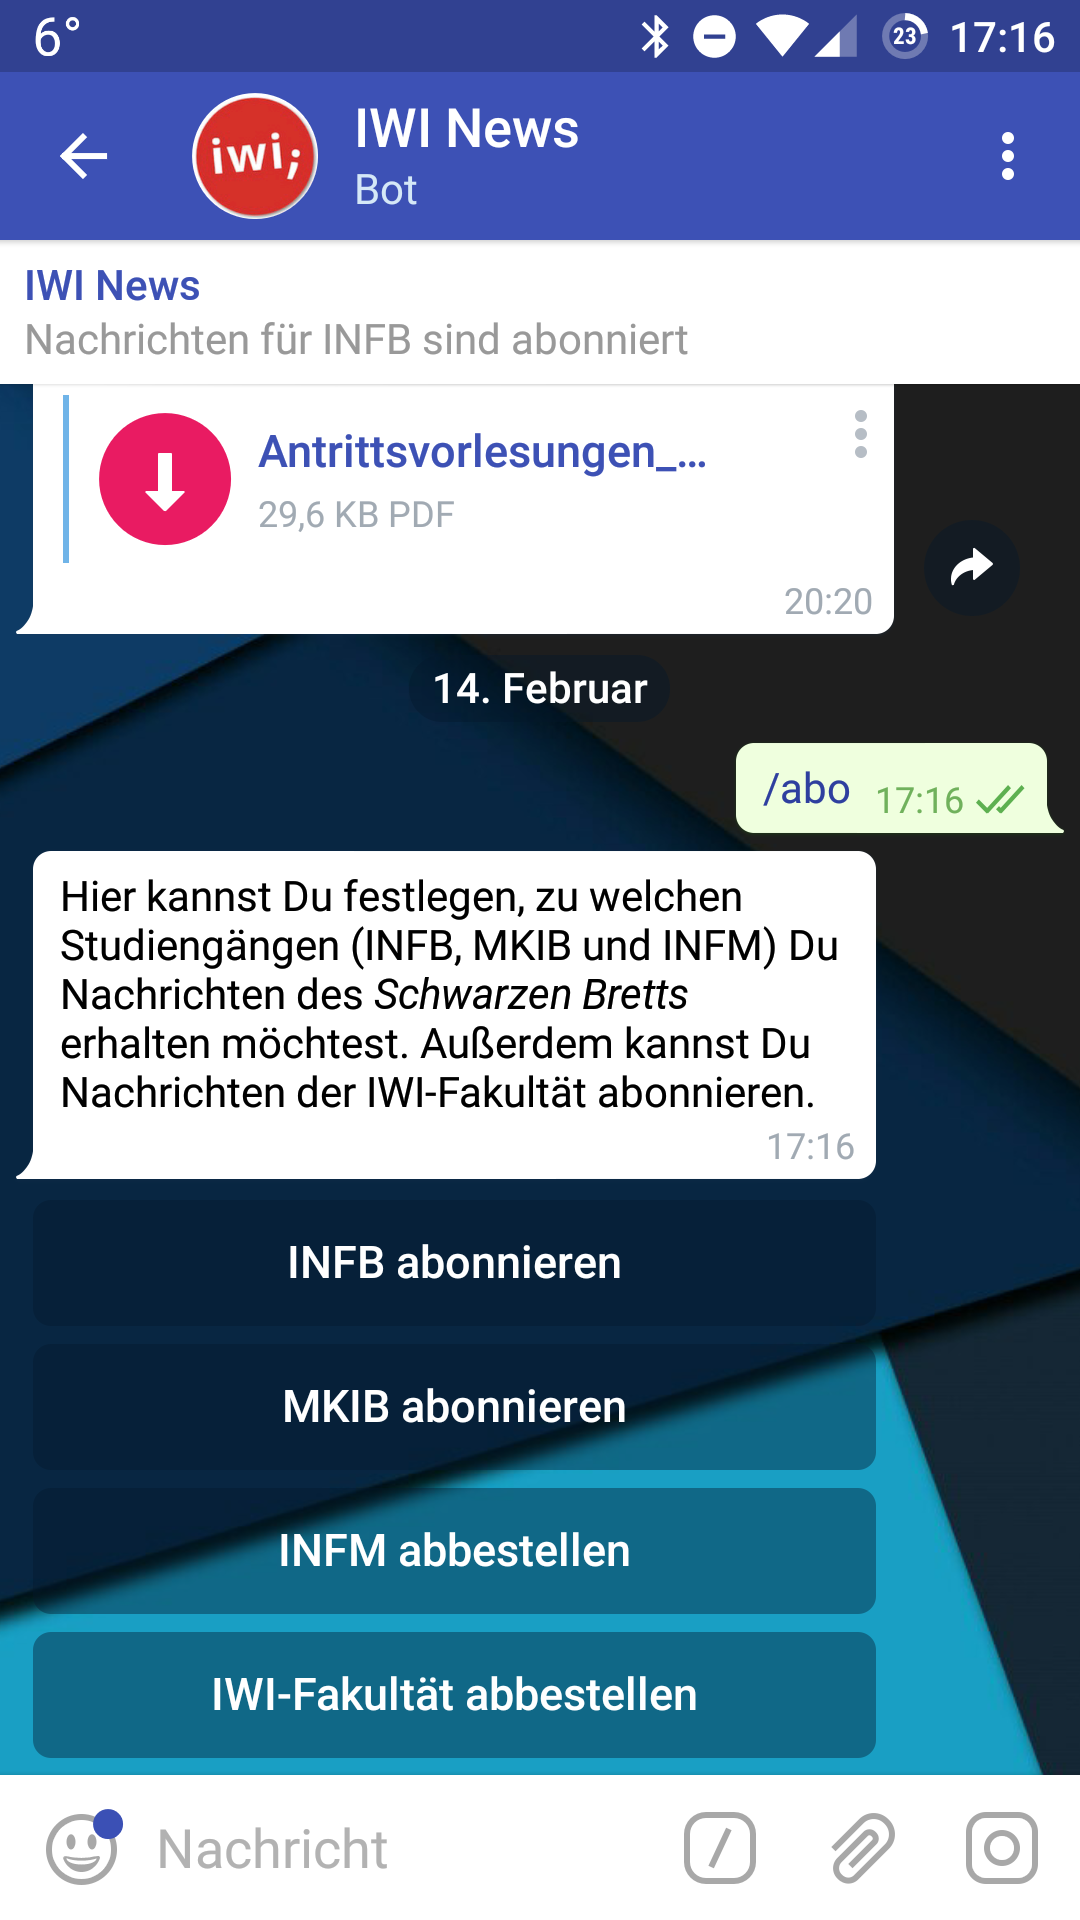
\includegraphics[width=0.4\linewidth]{SettingNotification.png}
      \label{img:notification}
    \caption*{Quelle: Eigene Abbildung}
\end{figure}

\subsection{Die weiteren Kommandos}
Alle weiteren Kommandos sind mit den bereits vorgestellten Methoden umgesetzt worden. Aus diesem Grund werden diese nicht detailliert vorgestellt.

Nur das \texttt{/settings}-Kommando sticht durch seine andere Usability hervor, hier kann der User den angezeigten Mensapreis anpassen. Es gibt 3 Preis-Optionen, die in~\autoref{sec:Funktionsumfang} bereits vorgestellt wurden. Eine solche Option würde man klassisch über ein Drop-Down Menü darstellen, in diesem Szenario wurde jedoch ein Inline-Button gewählt, der über alle 3 Optionen toggelt und über eine Benachrichtigung die aktuelle Auswahl erklärt.

\section{Hintergrundsynchronisation}
Im Hintergrund wird permanent nach neuen Einträgen gesucht, dies geschieht in der Klasse \texttt{BackgroundFeedSync}.

\begin{lstlisting}[language=scala, style=scala, caption={Start Methode der Klasse BackgroundFeedSync}]
/**
  * The background sync task is started by calling this method. Since this starts the
  * background tasks, it should be
  * noted, that calling this method multiple times will yield too many calls to the feed's
  * servers and should be avoided.
  */
def start(): Unit = {
  // Start searching 10 seconds after launch and then every 2 minutes
  backgroundActorSystem.scheduler.schedule(10 seconds, 2 minutes) {
    logger.debug("Loading remote data.")
    val entries = feedProcessor.receiveEntries()
    val facultyNews = feedProcessor.receiveFacultyNews()
    logger.trace(s"Received ${facultyNews.size} faculty news items")
    val newEntries = saveEntries(entries)
    val newFacultyNews = redis.addFacultyNews(facultyNews)
    newFacultyNews.foreach(news =>
      logger.info(s"""New Faculty News received: ${news.hashCode4DB()}
        |${news.title}
        |${news.publicationDate}
        |${news.description}""".stripMargin))
    val subscriptionEntries = entriesForSubscribers(newEntries)
    val subscribedFacultyNews = subscribedFacultyNewsUsers()
    logger.trace(s"Received ${subscribedFacultyNews.size} faculty news subscribers")
    sendPushMessageToSubscribers(subscriptionEntries)
    // This is the original method, but in order to avoid sending out outdated faculty news,
    // the new faculty news gets replaced by an empty list, which will result in no messages sent.
    // sendFacultyNewsToSubscribers(subscribedFacultyNews, newFacultyNews)

    // Debug purpose
    sendFacultyNewsToSubscribers(subscribedFacultyNews, List())
    newFacultyNews.foreach(news =>
      notifyAdmins(s"New faculty News entry with Hash ${news.hashCode4DB()}"))

  }
}
\end{lstlisting}

Direkt zu Beginn wird das Actor System \texttt{backgroundActorSystem} als Hintergrundprozess definiert, der nach 10 Sekunden und dann alle 2 Minuten gestartet werden soll. Hierbei werden zuerst alle Nachrichten des Schwarzen Bretts bezogen, danach die Fakultätsnachrichten. Diese Nachrichten werden der Redis-Datenbank hinzugefügt, hierbei wird überprüft, welche Nachrichten tatsächlich neu sind und diese werden dann zurückgegeben. Im Anschluss werden die Subscriber aus der Datenbank geholt und an diese werden die Nachrichten verschickt.

Da es Probleme mit den Fakultätsnachrichten gab, werden diese momentan nicht verschickt, es wurden in der Vergangenheit Nachrichten als neu erkannt, obwohl diese nicht neu waren. Die Ursache hierfür ist bislang unbekannt, es werden aus diesem Grund mehr Informationen geloggt.

Ein möglicher Grund ist, dass die Fakultätsnachrichten keine eindeutige ID haben, worüber sie identifiziert werden könnten. Um zu prüfen, ob eine Fakultätsnachricht neu ist, wird zur Zeit ein Hash der Nachricht berechnet und in der Datenbank gespeichert. So kann für jede Nachricht geprüft werden, ob diese bereits existiert, oder aber neu ist. Es wird hierbei der sha256 Hash genutzt und es werden der Titel einer Nachricht und deren \texttt{publicationDate} gehasht.

Die Nachrichten des schwarzen Bretts hingegen, verfügen über eine eindeutige ID, somit kann über diese ID einfach geprüft werden, ob es sich um eine neue Nachricht handelt.

Hat ein Nutzer mehr als einen Fakultätskanal (INFB, MKIB, INFM) abonniert, so soll dieser nicht mehrere gleiche Nachrichten erhalten, falls diese Nachricht in mehreren Kanälen gepostet wird. Somit werden vor dem Versand Nachrichten-Duplikate eliminiert, siehe~\autoref{code:entriesForSubscribers}.

\begin{lstlisting}[language=scala, style=scala, caption={Verteilung der Nachrichten auf die Subscriber und Eliminierung von Duplikaten}, label={code:entriesForSubscribers}]
def entriesForSubscribers(entries: Map[Course, Set[Entry]]): Map[UserID, Set[Entry]] = {
  val userConfig = redis.userConfig().filter(_._2.isDefined).mapValues(_.get)
  userConfig.map {
    case (userID: UserID, subscribedCourses: Set[Course]) => {
      val coursesForUser = mutable.Set.empty[Entry]
      entries
        .filter(e => subscribedCourses.contains(e._1))
        .foreach(e => e._2.foreach(entry => coursesForUser += entry))
      (userID, coursesForUser.toSet)
    }
  }
}
\end{lstlisting}

Zuerst wird hierfür die Konfiguration aller User aus der Datenbank geholt. Dann wird für jeden User geprüft, welche Kanäle er abonniert hat. Nun wird geprüft, ob neue Nachrichten für diesen Kanal dabei sind. Das Ergebnis ist eine große Map, in der jeder User eine Liste von neuen Nachrichten erhält, die ihm dann vom Bot zugeschickt werden.
